% ICMC 2006 paper template for Latex2e.

% Points to note:
%    Please use \paragraph instead of \subsubsection -- see discussion below.
%    See comments in the References section on how to do citations.

\documentclass[10pt,letterpaper]{article}
%\usepackage[]{natbib}
\usepackage{fullpage}
\usepackage{times}
\usepackage{chicago}                    % for "(Author, year)" cite style.
\usepackage{indentfirst}                % indent para after headings.
%\usepackage[pdftex]{graphicx, color}
\usepackage{graphicx, color}
\usepackage{url}                      % (handy if you reference a URL.)
\makeatletter
\def\url@leostyle{
  \@ifundefined{selectfont}{\def\UrlFont{\sf}}{\def\UrlFont{\small\ttfamily}}}
\makeatother
\urlstyle{leo}

\setlength{\oddsidemargin}{-0.25in}     % Latex has one-inch "driver margin"
% \setlength{\evensidemargin}{-0.25in}  % (shouldn't be necessary)
\setlength{\textwidth}{7in}             % 8.5 - 2*0.75 

\setlength{\columnsep}{0.25in}
\setlength{\parindent}{0.2in}

\raggedbottom                           % better than inter-para spaces, I say.


\begin{document}

\twocolumn

\title{\textbf{Negotiating the Musical Work. \\An empirical study.}}
\author{
Henrik Frisk and Stefan \"{O}stersj\"{o}\\
Malm\"{o} Academy of
Music - Lund University \\
henrik.frisk@mhm.lu.se\\
stefan\_ostersjo@hotmail.com\\
}
\date{}     % no date
\maketitle

\pagestyle{empty}          % no page numbers.
\thispagestyle{empty}      % yes, that includes not on the first page, either.

% do abstract by hand -- \begin{abstract} wouldn't conform to the guidelines.

\begin{center}
\large{\textbf{Abstract}}

\end{center}
% there's this annoying little indent here I can't properly eliminate, so...
\hspace*{-0.1in}                       % hackily cancel it out.
\noindent
\textit{
In this paper we explore the inter-relations between performer and
composer through two empirical studies and the result of this work is 
intended to lay the
ground for a new work for guitar and computer by Henrik Frisk for
Stefan \"{O}stersj\"{o}. By better understanding the composer-performer
interaction we also hope to better understand the necessary conditions
for a successful performer-computer interaction. We approach the issue
using a semiological approach and a qualitative method. In the works
studied we find reason to suggest that composition as well as performance interpretation oscillate between constructive and interpretative
activities. From this we draw some conclusions that we will attempt to
develop and implement in the upcoming collaborative work.
}

\section{Introduction}
This article discusses the musical work prior to its ultimate notation
and prior to its performance; we discuss the musical work in the Western
art music tradition, specifically music for solo instrument and live
electronics. In lack of a general terminology we use the term 'mixed
media' in this article to refer to a work for instrument(s) and
electronic sounds. By mixed media music we refer to music in which
sounds produced on acoustical instruments are mixed with sounds from
electronic sources or electronically processed versions of the acoustic
sounds played back on loudspeakers. One medium of sound production
(acoustic instruments) is mixed with another (loudspeakers). This
project is part of our respective artistic research projects at the
Malm\"{o} Academy of Music, Lund University and is an effort to combine
reflection, analysis, and empiricism in the framework of artistic
research.

Our purpose is to acquire a deeper understanding for the underlying
processes in the communication between the composer and the performer
and the social significance traditionally assigned to these roles in
relation to their operative significance. By better understanding the
interaction between the two parties involved in the creation of the
work, we also hope to better understand the necessary conditions for a
successful interaction between the performer and the electronics.
Obviously one of the fundamental conditions for a study such as this is
that the performer and the composer are both alive, and that the
performer has a genuine interest in performing the work in question.

\subsection{Music and notation} \label{twoagents}
The invention of notation has not only given us the notion of the
musical work but has also resulted in a split of 'the musician' into two
agents, composer and performer \cite{wis96}. A musical work, in the cultural context
of the Western art music tradition, is commonly regarded as the result
of a process in two distinct phases; one constructive and one
reproductive \cite{nattiez}. The composer produces a score, which in turn is handed
over to a performer who makes an interpretation of the notation and
reproduces it as specified in the score, hopefully quite faithfully to
the composer's intentions. The notation constitutes the primary source
of information. According to the line of thought in Paul Ric{\oe}ur's
hermeunetic philosophy, the traditional view of the author as a one-way
sender of a message is disputed - the author is disengaged from the work
by the act of writing \cite{ric91} (See also \cite{barthesMus}\nocite{barthes1}). Similarly, we suggest that the construction
of a score-based work consists of dialectic interplay between creation
and interpretation, in which the composer, at times, has to approach his
own notation by means of interpretation, even during the act of
writing. On the other hand the performer does not merely reproduce the
work such as notated, performing a score-based work is a co-creative act
in which the performer necessarily has to make crucial artistic
choices \cite{kivy,davies}. In other words, notation does not divide composer and performer
into one originator (producing the work) and one interpreter
(reproducing the work). Interpretation is a part of both creative acts.

\section{Method}
\subsection{Semiological approach}
Musical semiology has been constructed with the intention to provide
tools for analytical understanding of the musical work in its entirety
including the socio-cultural context. (For an excellent overview of the history of musical semiology \cite{nat89}.)
Attempting to move to a lower level of organization than that of musical notation may help to
further clarify the issue in relation to a wider sphere of
knowledge. (See Umberto Eco's discussion in \cite[pp.372]{eco71}).

\paragraph{The three dimensions} \label{threedim}

Molino reminds us that the hypothesis that there is a 'single,
well-defined item of information to be transmitted, all the rest being
simply noise' is 'dangerously inaccurate and misleading as soon as we
move from the artificial communication of information to a concrete act
of human communication as a total social fact.' Music, according to him,
is a product and not a transmission. Hence Molino suggests a model for
symbolic analysis on three levels; 'the poietic, the esthesic and the
'neutral' analysis of the object'. Three modes all representing the same
work of art. The poietic level is the constructive phase, the esthesic
is the interpretative phase and the neutral is the trace left by the
poietic (or esthesic) process \cite{molino}\nocite{molino2}. The
tripartite model for analysis has also been proposed by another of the most
important advocates for musical semiology, Jean-Jaques Nattiez:
\begin{quote}
...recognizing, elaborating, and articulating the three relatively
autonomous levels (poietic, neutral and esthesic) facilitates knowledge
of all processes unleashed by the musical work, from the moment of the
work's conception, passing through its 'writing down', to its
performance. \cite{nattiez}
\end{quote}
In the first empirical study in Section \ref{harp} we focus mainly on
the neutral level whereas in the second study (Section \ref{viken}) we
map the processes onto the poietic and esthesic levels of analysis.

\subsection{Qualitative method}
The video documentation from the collaboration between Love Mangs and
Stefan \"{O}stersj\"{o} consists of many hours of recorded data from
different occasions.  The selection of video clips to be analysed in the
present study was made on qualitative grounds, but not using the typical
method of theoretical sampling. The selection was
instead based on the pre-understanding ({\itshape
Vorverstehen})\footnotemark of 
\footnotetext[1]{We use the term pre-understanding as a translation of
Gadamer's notion of {\itshape Vorverstehen}; any kind of
interpretation (of texts) requires an anticipated understanding of the
analyzed object. \cite{gad60}}
\"{O}stersj\"{o}'s, having himself been part of the collaborative process. From his
knowledge of the sessions and the recorded material \"{O}stersj\"{o} suggested
some sections that he found especially interesting. This approach to the
analysis of video material generated in artistic research has been
previously discussed by \"{O}stersj\"{o} and Hultberg
\cite{ost05}. Similarly, the selections made for the other empirical
study was made based on Frisk's pre-understanding of the processes
leading up to the different versions of the material in that study.

\paragraph{Qualitative Method in machine-musician interaction}

The selected video clips were transcribed verbatim by Frisk and
\"{O}stersj\"{o} together. This turned out to be a very useful tool for
the sake of keeping a detached and relatively objective point of view on
the material. The transcription in turn was used as material for a graph
that became an important analytical tool in the study. It was only at
the point when the graph was produced that the implications of the study
on machine-musician interaction started to materialise.

\section{Empirical study} \label{empirical}
\subsection{Harp piece} \label{harp}
\paragraph{Introduction}
The work discussed here is a work in progress. It was commissioned by
the Mexican harpist Mercedes Gomez in 2004 for harp and computer. The
melodic material used for the piece consists of a small six note
fragment that is transposed and repeated creating a tone row of
potentially infinite length. Due to the cromaticism of the series the
material isn't very idiomatic for the harp. It was chosen because of its
inherent structure and its relation to the original vision of the
music. But also because of a genuine interest for the process of
negotiation between the fundamental building blocks of the composition
and the idiomatics of the instrument for which the composition is
intended. The process of adapting this specific material for the harp will
inevitably involve constructive interpretation, performed by the
composer on his own musical idea. In the case of the bars discussed below, much of
these negotiations were discussions between Frisk and the performer.
%Expressed differently we could say
%that the composer is working in the esthesic domain on the trace left by
%the poietic act of generating the first molecules of the evolving
%piece.
It is important to bear in mind that to some extent the notion of what
is ``idiomatic'' and ``playable'' is relative to the technical approach
and instrumental modes of expression of a certain performer. Naturally,
many of the solutions and suggestions below relate very specifically to
this collaboration and cannot be generalized as such.  A certain amount
of dialogue between idiomatics and musical ideas is likely to occur in
any kind of compositional work but the conditions under which this work
in progress has evolved makes the internal as well as the external
negotiations stand out.

\paragraph{Analysis}
The following is a discussion on four notations of the same two bars of
music. The first (Figure \ref{harpex1}) is the original idea transcribed
as closely as is meaningful into the atomized rhythmic structure of
western notation. The basic musical idea at this spot is to have the
same variation of the tone row in three individual parts, separated by
octaves, each one following its own unique and precisely notated
rallentando.
\begin{figure}[!htp]
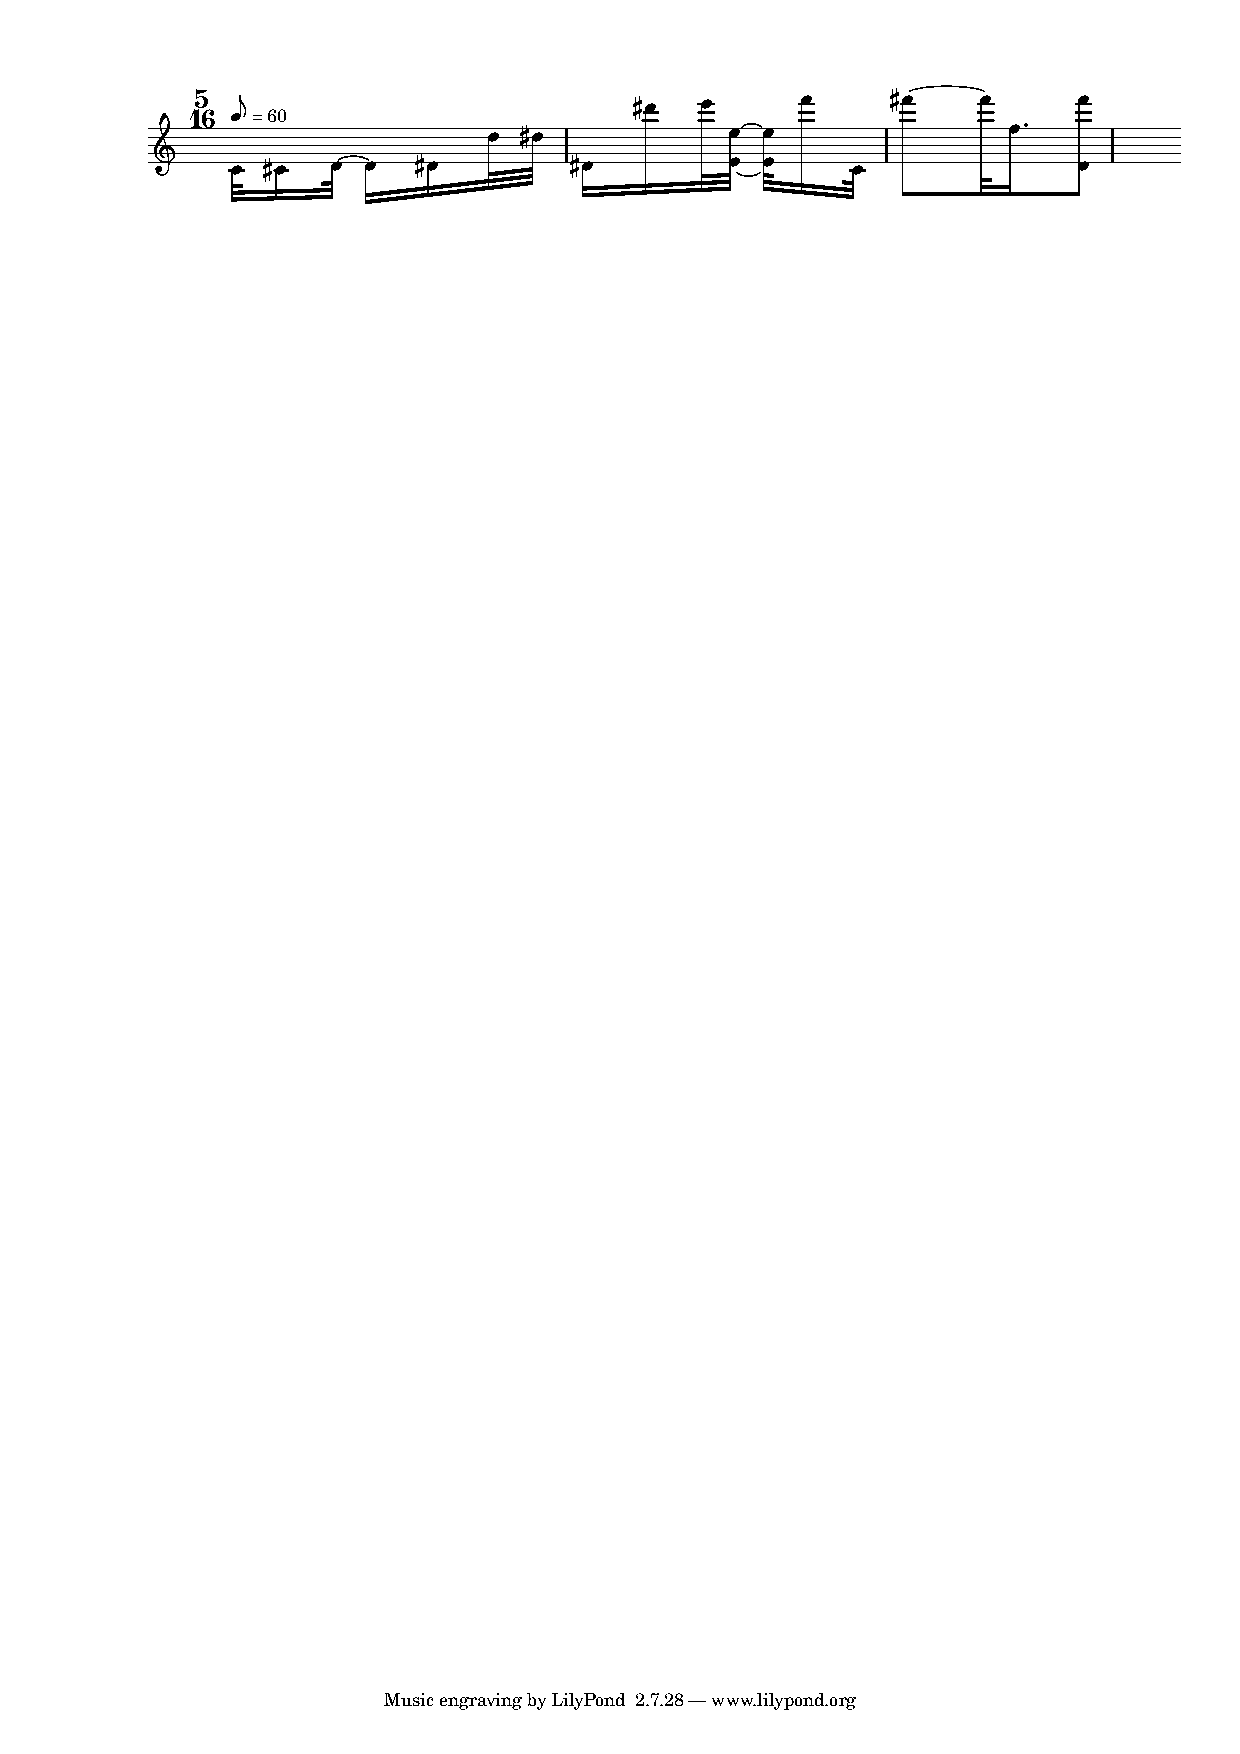
\includegraphics[width=1.0\columnwidth]{img/harpVersion1}
\caption{First transcription of the idea into notation.}
\label{harpex1}
\end{figure}

In the second example (Figure \ref{harpex2}) we find the first attempt
at transcribing the musical idea for the harp. Pedal changes are not
notated. At the indicated tempo, these two bars are still virtually
unplayable on the harp. The F flat to F natural pedal change at the end
of the first bar is a technical problem as is the G flat to G natural on
the second eighth note of the second bar. After working on this passage
with the harpist a version in the lines of Figure \ref{harpex3} was
suggested.


\begin{figure}[!hbp]
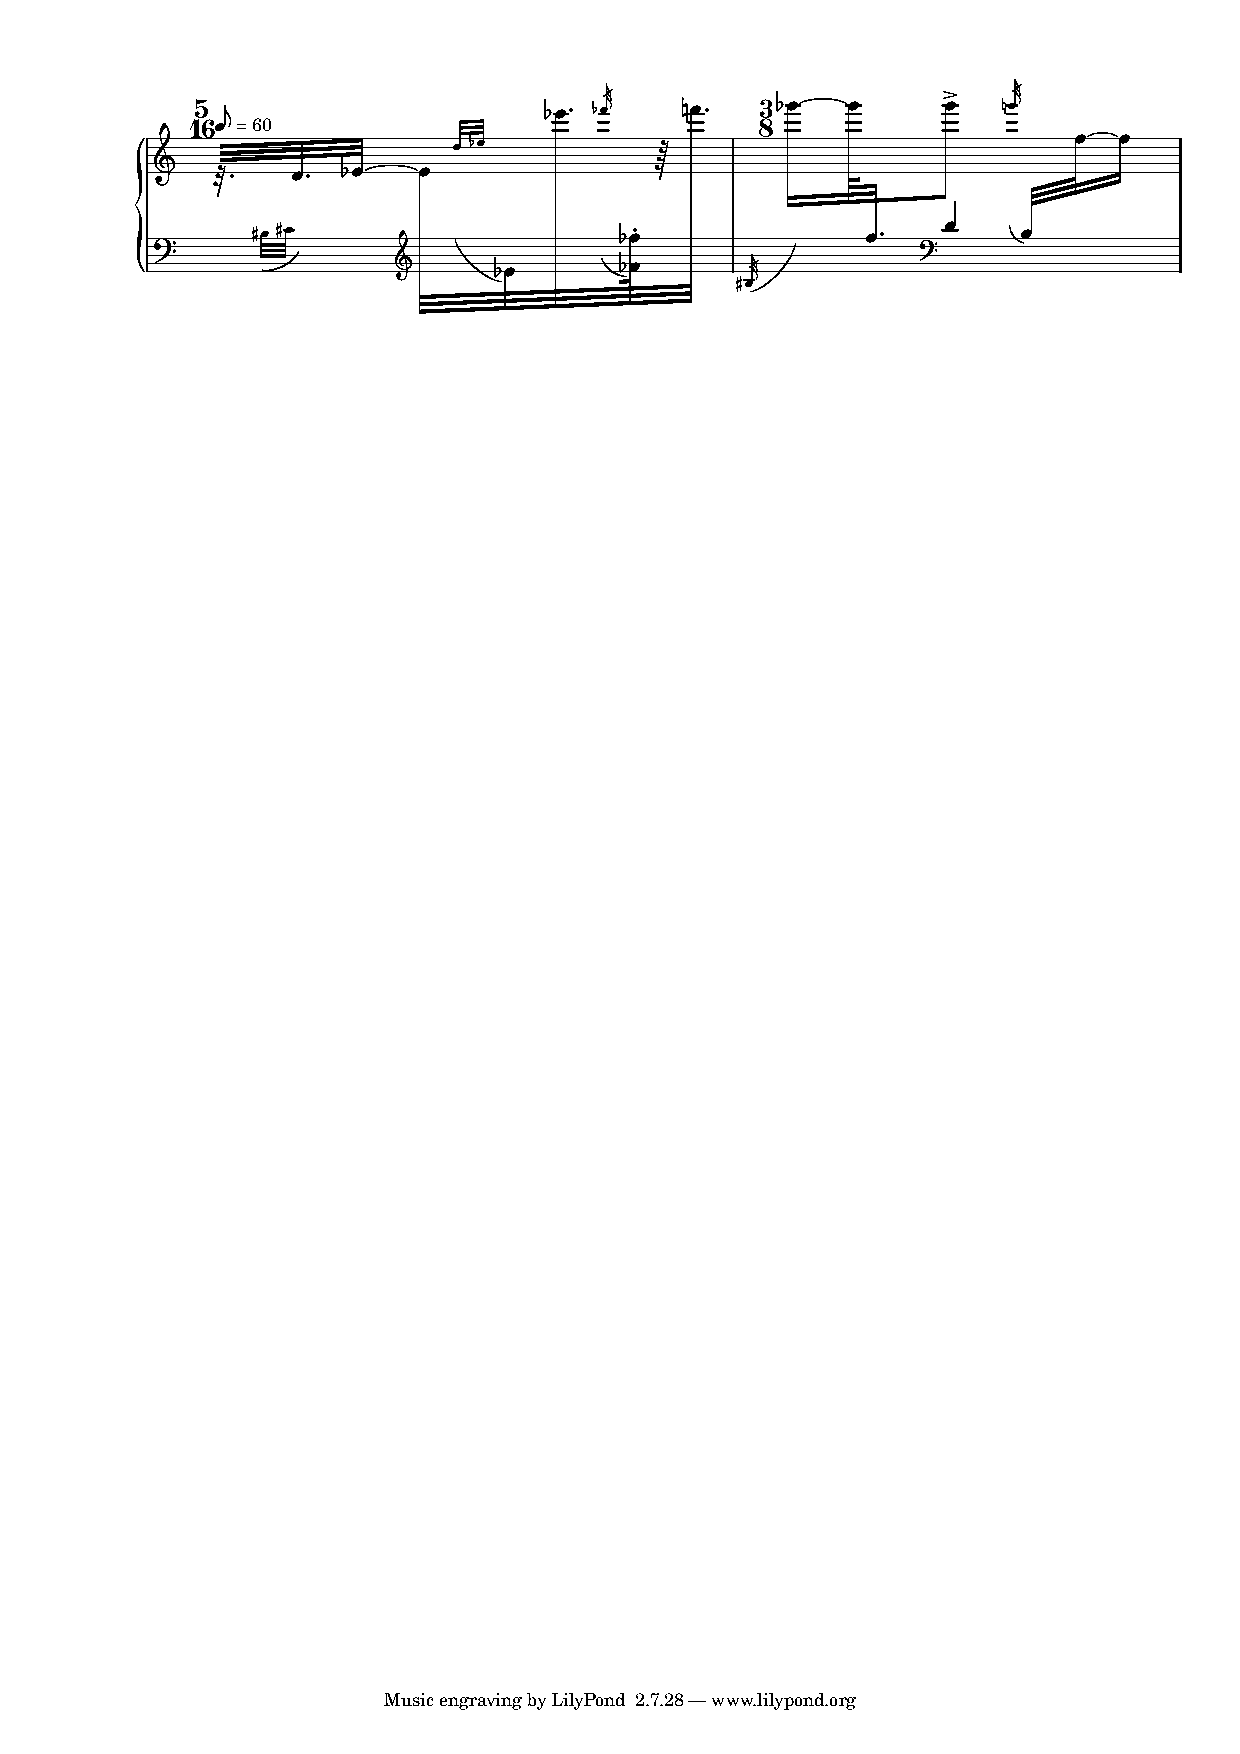
\includegraphics[width=1.0\columnwidth]{img/harpVersion2}
\caption{First transcription for the harp.}
\label{harpex2}
\end{figure}

The third example (Figure \ref{harpex3}) is rhythmically less
complex. With a few written indications the effect of the slowing down
of the music could be approximated. The pedal changes are resolved by
means of pedal glisses. However the independent parts and their
individual rallentandi cannot be traced in the image that this notation
produces, which also means that a neutral analysis of this version will
reveal little of the original intentions.

\begin{figure}[!ht]
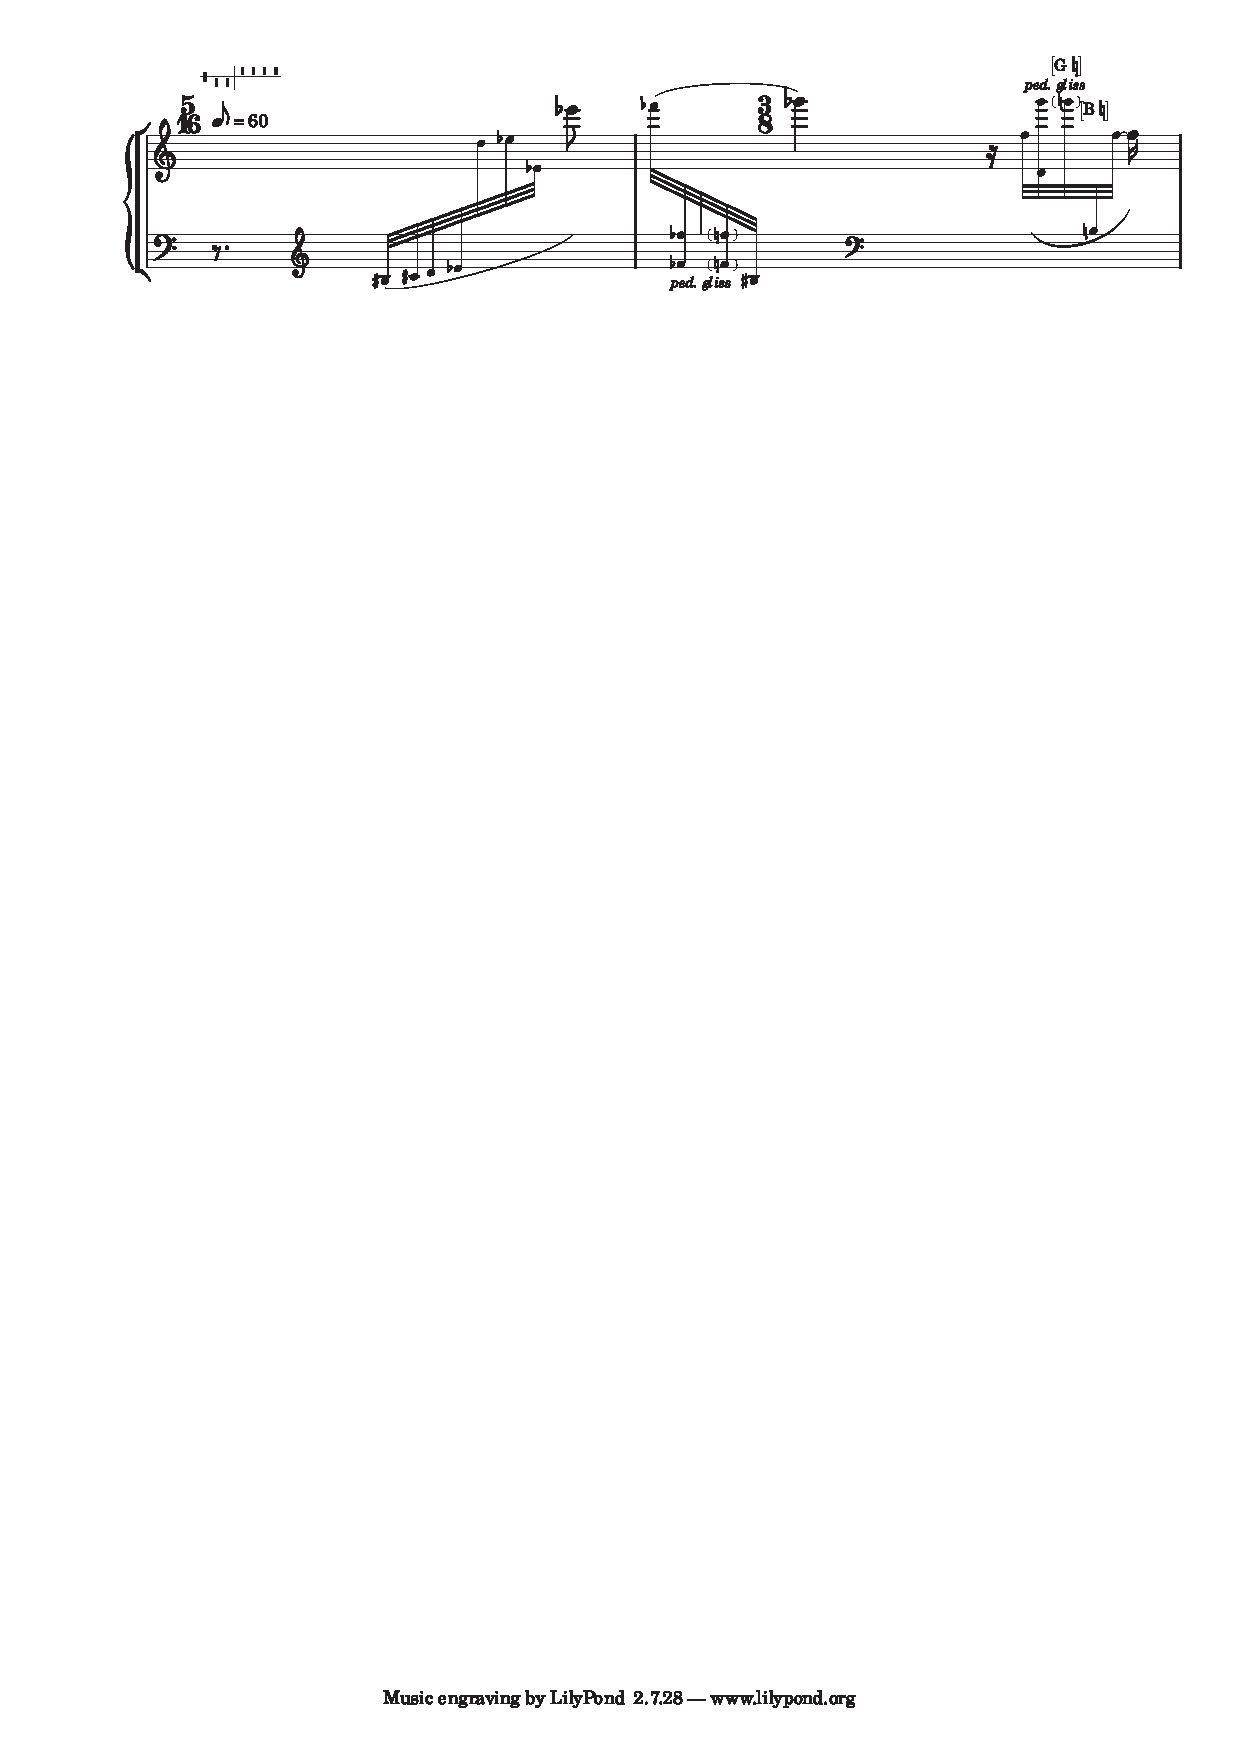
\includegraphics[width=1.0\columnwidth]{img/harpVersion3}
\caption{A transcription rhythmically less complex.}
\label{harpex3}
\end{figure}

In the final example some of the rhythms have been simplified by use of
grace notes and, as in the previous example, some of the pedal changes
have been changed into pedal glissandos. This contributes to making the
idiomatics of the instrument a part of the counterpoint and a
balance, acceptable by both the composer and the performer between
``authenticity'' (to the original idea) and the playability of the
excerpt, has been reached.

\begin{figure}[!htb]
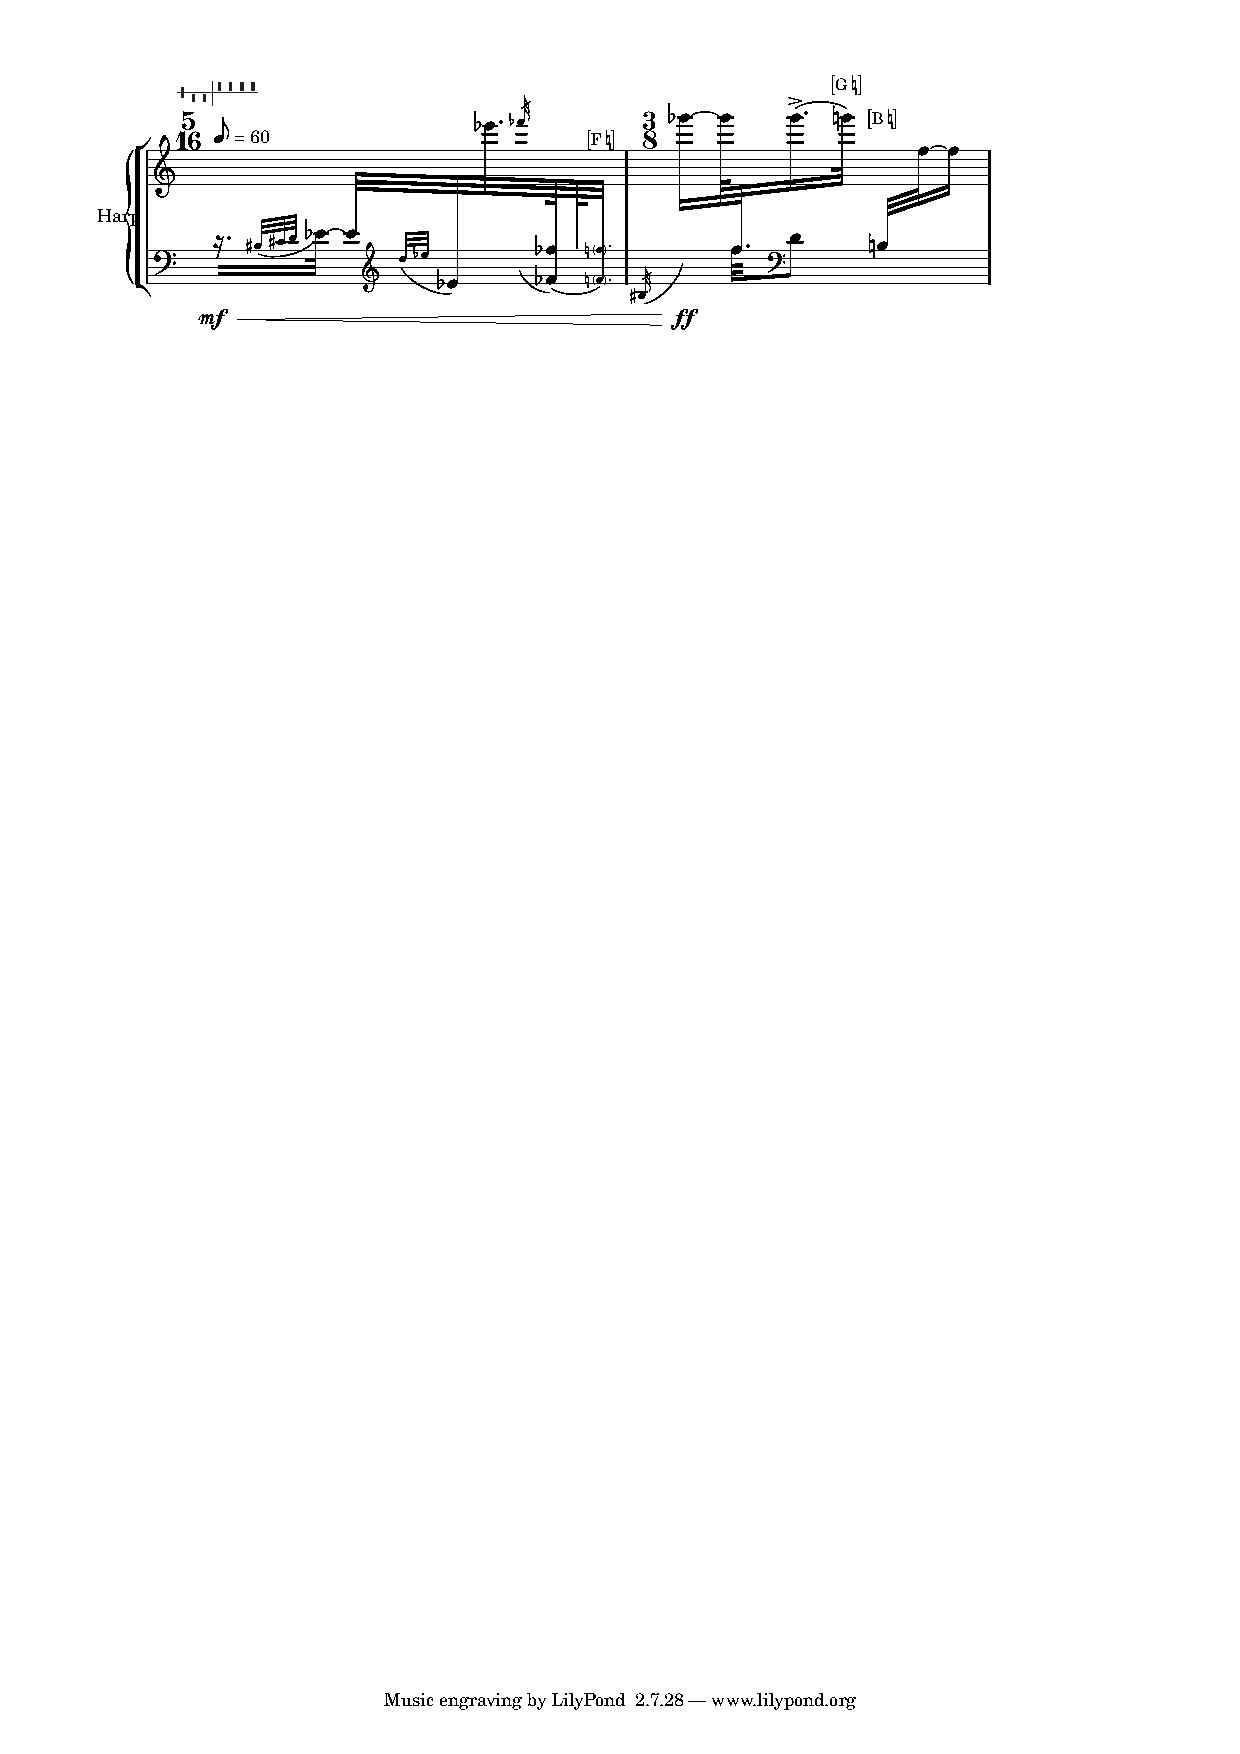
\includegraphics[width=1.0\columnwidth]{img/harpVersion4}
\caption{A final version. More idiomatic than the example in Figure
\ref{harpex1}, but closer to the original idea than Figure
\ref{harpex3}} \label{harpex4}
\end{figure}

\paragraph{Conclusions}
Considering the esthesic processes in the evolving notation of this
passage in the light of the discussion in Section \ref{twoagents}, it
might be worthwhile to consider the significance of Frisk's conceptual
vision of the work and how the negotiations between this musical matter
% (immaterial as it may seem) 
and the idiomatic constraints of the harp lead up to a version of the
work in musical notation. And further, how the presence of the performer
in this discussion provides new impulses for the piece, specifically its
notation and rhythmical articulation. The original vision is the trace
that constitutes the source for the interpretative, i.e. esthesic,
actions leading to the different notations. Though the notation is
altered significantly through the four variations the core of the
original musical vision remains the same throughout the different
varitations; i.e. on the poietic level the negotiations did {\itshape
not} alter the music. However, in a neutral analysis of these four
excerpts we might be tempted to suggest that the process lead to four
different kind of musics. In any event, we find that the study shows the
recursive nature of the interplay between constructive (poietic) and
interpretative (esthesic) processes both in the communication between
the composer and the performer, but also as an internal process in which
the composer himself is negotiating between the original vision and its
representation in musical notation.

%
%In this context 'the work' is
%the conceptual vision, in whichever way it comes to the
%composer. However, as the following analysis shows, it makes little
%sense to isolate one certain point in this process claiming that it
%alone should make up 'the work'. Rather, it seems fair to assume that
%the musical work is the product of a complex chain of poietic and
%esthesic processes working together in an infinite loop.
%
%
%A musical work is the product of
%a complex chain of poietic and esthesic processes, which starts out with
%the conceptual vision, in whichever way it comes to a
%composer. 
%
%It seems
%to us that it makes no sense to isolate one certain point in this
%process claiming that it alone should make up 'the work'.
%
%Referring to the discussion above, the transformation that these two
%bars of music goes through would imply that the composition is neither
%the acoustic trace left by the performance nor is it the score. It is
%the conceptual idea, the vision, of the work as it is envisaged by the
%composer. Everything else, including the notation of the music, are
%creative interpretations of this first and original notion of the work.


\subsection{Viken} \label{viken}
\paragraph{Introduction.}

Love Mangs' (L.M.) ``\emph{Viken}'' for guitar, banjo, e-bow and electronics (2004-05) was
commissioned for Stefan \"{O}ster\-sj\"{o} (S.\"{O}.) by the Swedish Arts Grants
Committee. The project had several explicit intentions, apart from the
mere production of a work for guitar and electronics. One was to use
real time processing as the main source of electronic sound, the other
was to explore the boundaries between composing and performing; between
the performance interpretation of a work and how different kinds of
fixity can be established in a work. This should be taken into account
when studying the video documentation of this process. It would be a
mistake to regard the material as documentation of a typical
collaboration between a composer and a performer, as both L.M. and
S.{\"O}. were well aware of the underlying intention to explore the
possibilities for improvisation and other interactive ways for composer
and performer to approach the process of creating a score-based work
with electronics. While studying the video it is also of importance to
remember that both parties involved are aware of their process being
documented. However, the session is taking place less than two months
prior to the scheduled premiere which implies that both parties are
strongly focused on the task of getting the piece together.

The transcription has played an important methodological role in our
analysis and can be found at
{\url{http://www.henrikfrisk.com/documents/vikenTranscript.pdf}}\newline
and all references in this text to the video refers to sections of the
transcription. The video clip is edited; sections with little or no
action are simply removed but the order of events are not altered. A
compressed version (QuickTime movie) of the edited video can be found at
{\url{http://www.henrikfrisk.com/documents/vikenMovie.mov}}. For
reference, an un\-edited version of the same passage can be found at
{\url{http://www.henrikfrisk.com/documents/viken-noEdit.mov}}. The
video was recorded during a session in the composer's studio on
September 17, 2005.

\paragraph{Material worked out prior to the documented session.}

It is of importance to the analysis of the communication processes in
the video to understand the material that L.M. and S.{\"O}. had at the
outset of the session. L.M. had derived a melody from a filtered
electronic sound clip, which originally wasn't intended for
``\emph{Viken}''. As the process of composing ``\emph{Viken}'' evolved
he wanted to include the sound file as well as the melodic material
derived from it in the work.  Almost any kind of notation will
inevitably be a reduction of the material that is the object for
notation. Already when L.M. decided to make a transcription of the sound
clip he subjectively chose elements to emphasize and elements to
exclude; thus making an interpretation of his own material. He is
working in the esthesic domain on the trace left by a work performed in
the poietic domain.

\begin{figure}
\begin{center}
\includegraphics[width=1.0\columnwidth]{img/viken} 
\caption{Love Mangs first notation of the melody derived from the sound file.}
\label{vikentrans}
\end{center}
\end{figure}

What is interesting with the way L.M. has carried out the transcription
is that he doesn't even try to establish a connection between the sound
clip and its expressive qualities in the notation. Instead he has
extracted an ordered set of discrete pitches that establishes a clear
tonality (see figure \ref{vikentrans}). We can
say that he re-constructed a musical motif independent from its
source. In the context of his working on ``\emph{Viken}'', what he heard in
the sound clip was the melody. An action performed in the poietic domain
as a result of working with the material in the esthesic domain but with
'knowledge of the poietics of the work' as Nattiez would put it, the
work in this case, not being the context of the sound clip but the
poietics of ``\emph{Viken}''.

\paragraph{Analysis of the video.} \label{thevideo}

\begin{figure}[!hbp]
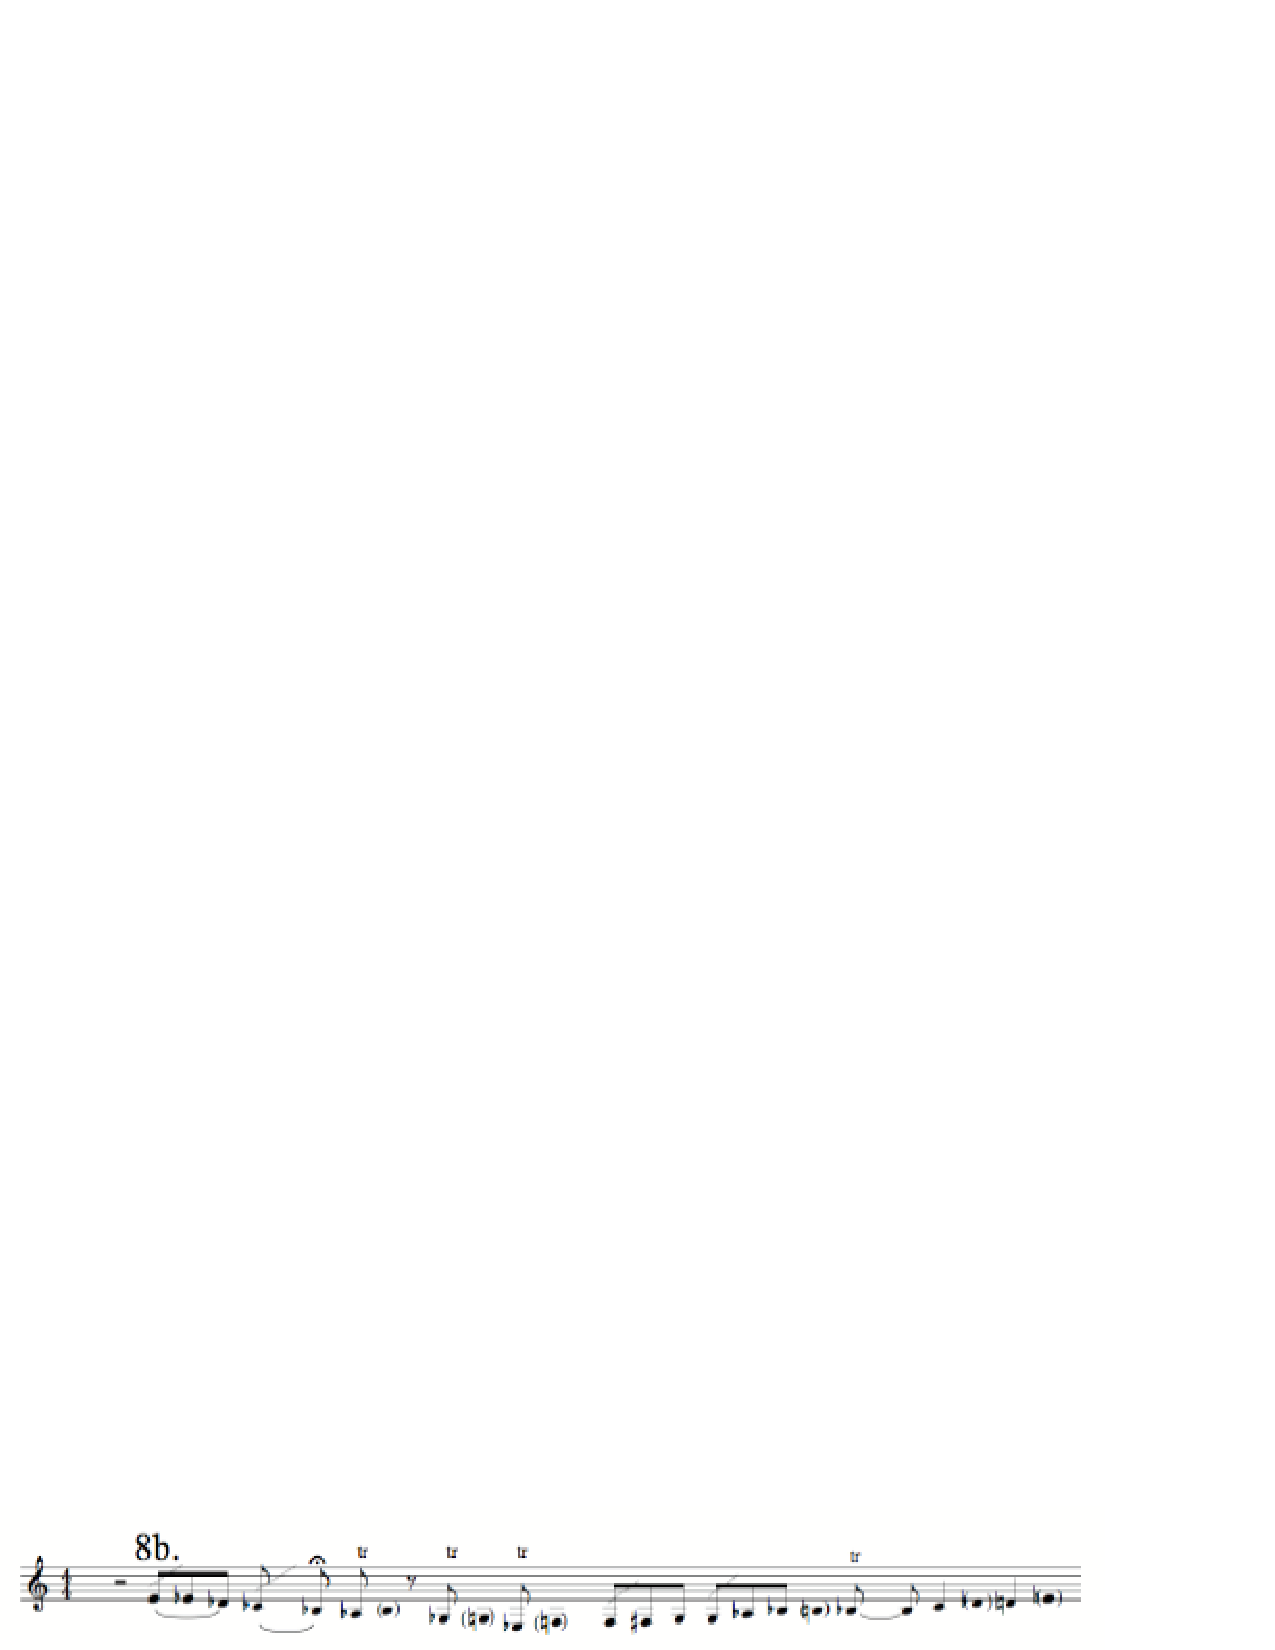
\includegraphics[width=1.0\columnwidth]{img/viken8b}
\caption{Material 8B from the final score of ``\emph{Viken}''.}
\label{viken8}
\end{figure}

The agreed purpose of the session documented in the video, was to work
out variations on the melody transcribed by L.M.. His intention was
to use this melodic material in the piece.

In the first scene S.{\"O}. has just played an improvisation on the melody
and on L.M.'s suggestion he is notating the new variation (see figure
\ref{viken8}). S.{\"O}. is active in the poietic domain, constructing new
material for the piece. He turns to L.M. for feedback, but at this point
L.M. appears remarkably indifferent. This is illustrated by the arrow
going from the \emph{new variation} box in the poietic field on S.{\"O}.'s
side of the graph pointing down towards L.M.'s side in figure
\ref{graph}.  There is a lack of communication between L.M. and S.{\"O}.
(illustrated by the dotted arrow going upwards from the \emph{restless,
passive} box) as L.M. does not respond to S.{\"O}.'s invitation to discuss
the new variation. L.M. seems to have accepted the new material as it
was played initially and instead takes the initiative (illustrated by
the initiative axis going from S.{\"O}.'s side to L.M.'s), adopting an
interpretative approach on S.{\"O}.'s variation. L.M. is now active in the
esthesic field, suggesting to S.{\"O}. the addition of a fermata in the
variation (line 24) represented by the \emph{fermata} box in the
graph. Now there is apparent noise in the communication (represented by
the dotted arrow going from the \emph{fermata} box to the \emph{new
variation} box): L.M. appears to be unclear of where in the notation the
fermata should be.  This in turn leads to a misunderstanding by S.{\"O}.
(line 59), taking L.M.'s suggestion to mean several fermatas (dotted
arrow from the \emph{several} box to the \emph{fermata} box).  Our
interpretation of the dialog and the interaction here is that it takes
L.M. a while to find the right spot in the notation (by S.{\"O}.). He
seems to point at different spots in the score but in fact he is seeking
for the end of the phrase which is where he meant for the fermata to be.
Eventually L.M. points it out and for the first time a clear
communication takes place, illustrated by the two arrows in the graph
going in both directions (line 68 in the transcription). In this segment
both L.M. and S.{\"O}. are acting in the esthesic domain, L.M. in his
interpretation of S.{\"O}.'s notation and S.{\"O}. attempting to try out
L.M.'s suggestion. S.{\"O}.'s initial misunderstanding of the fermatas
seems to lead to the next initiative taken by S.{\"O}. and is illustrated
by the initiative axis going from L.M. to S.{\"O}. at 75. Again in the
esthesic field, S.{\"O}. suggests that long fermatas could be added to the
last notes of the phrase. At first L.M. doesn't get the idea at all
(line 78, dotted arrow going from the \emph{long fermatas} box to the
\emph{what?} box) but eventually approves of the suggestion (line 85,
solid arrow going in the same direction).\footnotemark 

\footnotetext[2]{In the final version of the piece the electronics end
the section discussed in the session with a massive fermata.}

This is followed by what seems to be an attempt on L.M.'s part to enter
the creative discussion or to reclaim the artistic initiative. The
response from S.{\"O}. is not related to what L.M. says (the dotted arrow
going from the \emph{4th string} box over to S.{\"O}.'s side in the graph
at line 94). The passage ends with S.{\"O}. playing the whole phrase again
giving L.M. a look at the end (\emph{glance} box at line 111) without
getting a noticeable response (dashed left bound arrow). It is obvious
that the communication in both directions is very noisy - this passage
is filled with unanswered questions and misunderstandings.

In the next clip S.{\"O}. is writing down the variation in more detail,
inserting L.M.'s idea of the fermata as a normative inscription (line
119). In that sense the initiative is on L.M.'s side, in spite of the
fact that S.{\"O}. is the physically active part with the writing. At this
point S.{\"O}. is not artistically involved, basically just making a note
of L.M.'s interpretative idea. L.M. then develops his idea of the
fermatas and their significance in this passage, still active in the
esthesic domain. The way we analyze this follows a model in which the
difference between creative actions in the esthesic and poietic domains
is a difference in what class of material the creative act refers
to. Nattiez defines these as the psycho-sociology of creation and
psycho-sociology of perception respectively \cite{nattiez}. L.M.'s discussion of the
fermata emanates from his perception of S.{\"O}.'s improvised new
variation at the very beginning of the video clip and is therefore to be
regarded as an esthesic process.

\begin{figure}[!hbp]
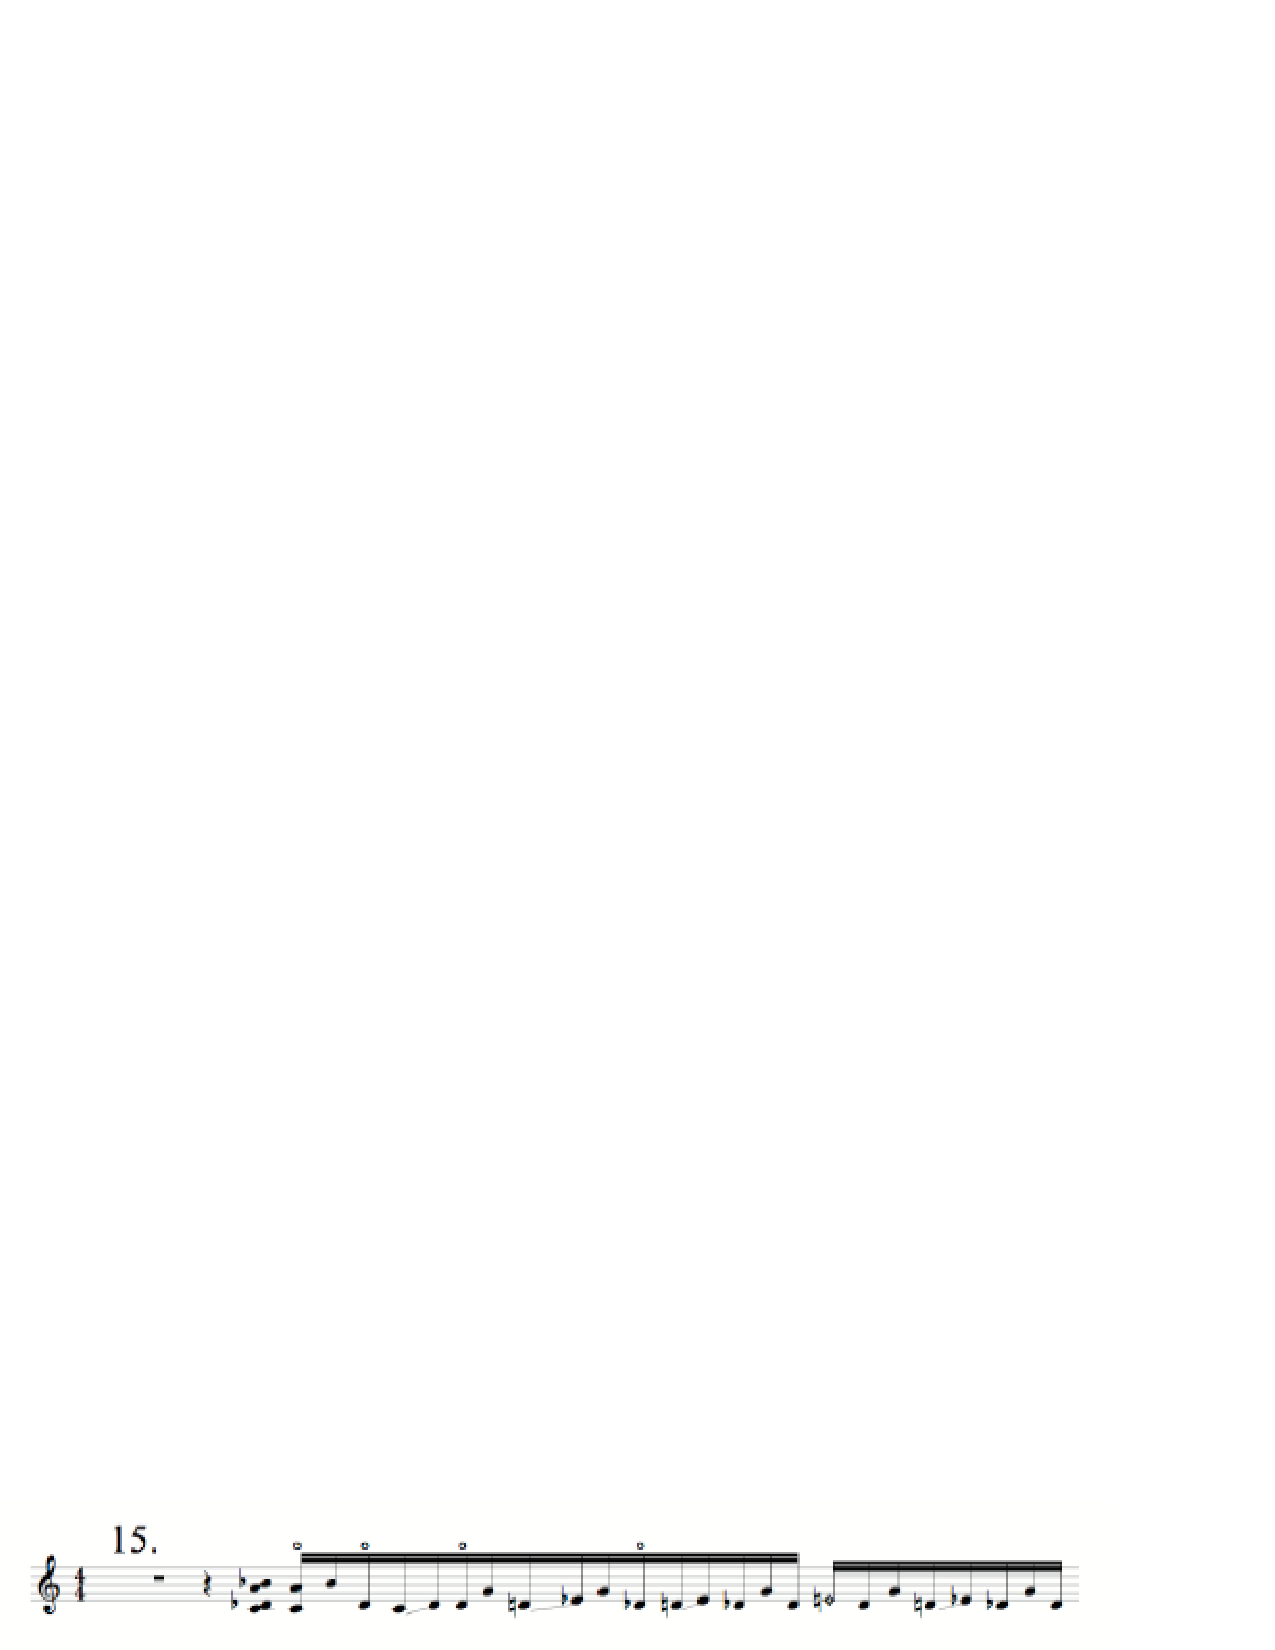
\includegraphics[width=1.0\columnwidth]{img/viken15}
\caption{Material 15 from the final score for ``\emph{Viken}''.}
\label{viken15}
\end{figure}

The idea of inserting several fermatas, which in the beginning was a
misunderstanding on S.{\"O}.'s side, is now completely accepted and
incorporated in the music as it is envisioned by L.M.. However, just as
in the previous passage, S.{\"O}. doesn't respond to L.M.'s
remarks. Instead he starts playing the phrase from the beginning (line
139) and, at the time he reaches the end of the phrase, introduces new
material in the form of an extended arpeggio (line 140). S.{\"O}. regains
the initiative and moves into the poietic domain. The communication at
the moment when the new material is discovered is immediate and
distinct; S.{\"O}. gives L.M. a glance and L.M.'s humming reply is
evidently positive (at line 145). At line 150 S.{\"O}. takes an
interpretative approach, commenting on the sound of the new
arpeggio. The clear communication at this spot is underlined by the
fact, that for the first time in the video clip, L.M.'s attention turns
to S.{\"O}. and the instrument and away from the music stand.

\begin{figure}[!ht]
\begin{center}
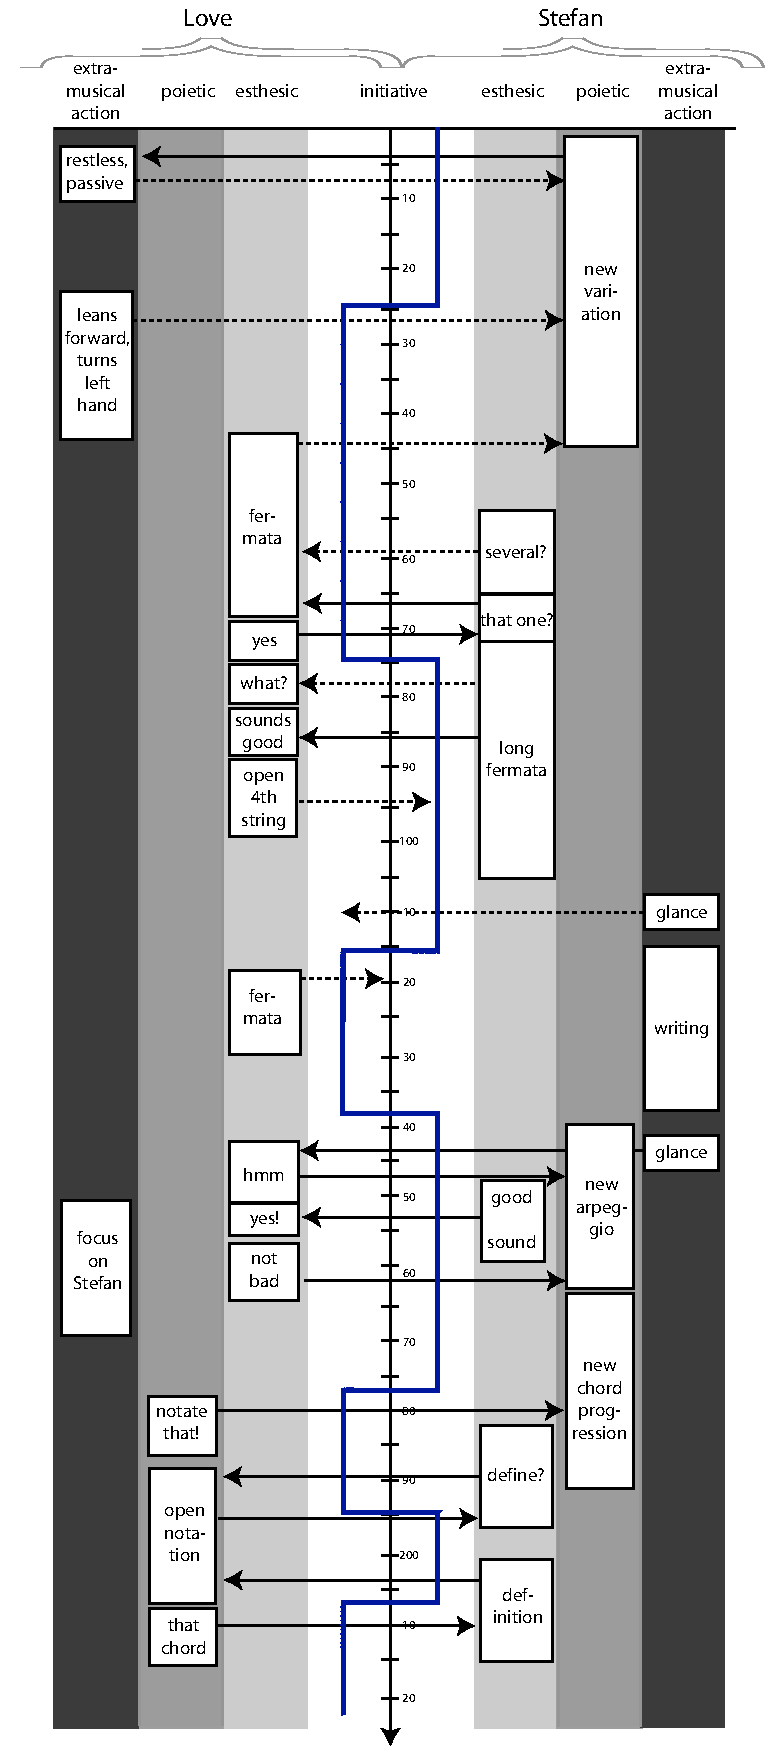
\includegraphics[width=0.8\columnwidth]{img/timeline_horiz}
\caption{A graph of the interaction between Stefan \"{O}stersj\"{o} and
 Love Mangs in the session analyzed in Section \ref{thevideo}. The scale
 in the center axis refers to line numbers in the transcription of the video.} \label{graph}
\end{center}
\end{figure}
%\thispagestyle{empty}

At this moment S.{\"O}. starts trying out a new context for the arpeggio
which evolved from the previous variation but is of a different
character.  He plays with the minor seconds that since the introduction
of the idea at line 140 have been leading up to the arpeggio and
attempts to merge the new arpeggio with a series of chords from L.M.'s
material notated prior to the session.  At this moment S.{\"O}. starts
to summarize the achievements so far during the day. He starts playing
the version of the melody with harmonics. L.M. interrupts him by asking
him to "notate the last thing you did!". The remark indicates that
L.M. has decided to include the new chord progression in his conception
of the piece (see figure \ref{viken15}) and thus his actions move into
the poietic field. This leads to a discussion on how to define the
passage in terms of musical notation. L.M. suggests that it doesn't have
to be all that defined ("Just notate it as a draft", line
201). S.{\"O}. suggests a strategy for the notation of the phrase which
L.M. finds satisfactory. In this last sequence L.M. is organizing the
material and performs a typical 'compositional' action still in the
poietic domain.

\section{Discussion}
% \begin{quotation}
%\begin{textit}
%{Just as the reading of the modern text consists not in receiving, in
% knowing or in feeling that text, but in writing it anew, in crossing
% its writing with a fresh inscription, so too reading this Beethoven is
% \emph{to operate} his music, to draw it (it is willing to be drawn)
% into an unknown \emph{praxis}.}
%\end{textit}
%\cite{barthesMus}
% \end{quotation}
\subsection{Whose work and whose performance?}

In the session with L.M. and S.{\"O}., the immediate impression for a
viewer could be that of a complete swapping of the agent's respective
roles: Who is the composer and who is the interpreter in the first video
clips? S.{\"O}. is writing music while L.M. is passively listening. L.M.
suggests the addition of a fermata in the variation that S.{\"O}. has just
notated. Our claim is that, even though we approach a situation in which
the relative positions happen to be at their respective extremes, what
we see is still within the boundaries of artistic practice both for
composers and performers. The observed interplay is an example of how
the roles of composer and performer in themselves overlap, and can even
seemingly be interchanged in this way.

In essence this is a matter of ontology: On the one hand, what makes up
the musical work, and on the other hand, what does performance
interpretation amount to? Just as was suggested in Section
\ref{twoagents} S.{\"O}.'s actions in the video clips involves a strong
element of construction. What performers do is making versions of works,
and these versions are in a sense the performer's co-creation of the
composer's piece.\footnotemark \footnotetext[3]{For a more elaborate
discussion on this topic see \cite{kivy} and \cite{ost05}.} But what
then defines the composer's work independent of its performances?
Following the line of thought of Stephen Davies, it is the
work-identifying instructions that delineates the work
\cite{davies}. For a musical work these instructions are usually
regarded to be some of the fundamental aspects of the notation. However
in Section \ref{harp} we observed how the work assumed a number of
different representations. In that case, though the notation will be
fixed and may eventually be said to constitute the `work-identifying
instructions' we will argue that the work does exist even prior to its
notation since, on the part of the composer, it makes up the reference
against which the negotiations are held. Furthermore in the case of a
piece for instrument and electronics, much of the identity of the work
is also specified in the computer programming and in the electronic
sounds. This is important to bear in mind while studying the session
with L.M. and S.{\"O}.. The point of departure is a melody that L.M. has
derived from a previous tape composition. The musical material that
evolved from L.M.'s transcription appears in a context where real-time
processing and pre-prepared tape material contributes strongly to the
identity of the music.

If we accept the idea that L.M. and S.{\"O}. are acting as composer and
performer respectively and consider how their actions can be divided
between the poeitic and esthesic fields, also taking into account the
discussion in Section \ref{harp}, we may draw some important conclusions
from the empiric studies:
\begin{itemize}
\item Composition may be regarded as a complex interaction between
      esthesic and poietic processes.
\item Performers may similarly be said to oscillate between these two
      modes of artistic activity.
\end{itemize}
What further follows from this is a possible contribution to the
semiological model of the musical work, with a more detailed
understanding of the esthesic and poietic processes at play in the
process of producing a score-based work in performance.

\subsection{Interactivity}
%One of the general difficulties in composing and performing music with
%live electronic elements is the difference in approach that the
%electronics seems to require when compared to a situation such as the
%one analyzed above. 

The flexibility that we can observe in the interaction between the two
agents in the video clip is remarkable. Complete misunderstandings and
miscommunication does not halt the process nor does it appear to lead to
false conclusions; it is only at a close examination of the flow of
events in the video that we can observe the misinterpretations. In the
end some of the misunderstandings, such as the idea of adding several
fermatas (line 59 in the graph, see figure \ref{graph}) worked their way
into the final version of the score.

The quote from Molino in Section \ref{threedim} can now be read in the
light of the performed analysis.  Although the misunderstandings can be
regarded as 'noise' when analyzed from the point of view of information
theory, in the collaboration between L.M. and S.{\"O}. it rather seems to
be an integral part of the artistic process. It shows how the classical
notion of the 'creative misunderstanding' really can play an important
role in artistic work.

The way the computer part in ``\emph{Viken}'' is set up, S.{\"O}. has
a pedal that controls the synchronization between himself and the
computer. This method of resolving that particular issue in mixed media
music is not uncommon. It relates to the notion of synchronization as
purely a technical issue; a unidirectional stream of
communication. Though the occasional pressing of a pedal does not
resolve the critical issue of rhythmic alignment and musical timing on
the micro level, it does keep the musics of the two parties aligned in
the larger structural meter. That is; when it comes to synchronization of
preprepared elctro-acoustic material with acoustic instruments what is
achieved is a series of meeting points and more seldom an integrated
flow of events.
Now, in the context of the composer/performer interaction (see the
analysis in Figure \ref{graph}) there is a striking lack of
synchronicity between the different actions. There is an evident and
independent flow of the initiative, of the constructive and of the
interpretative input between the two agents.
%Nevertheless, in the end the process leads to
%new material that is included in the final version of the piece.

Would it be possible to use the knowledge gained from the analysis of
the video in the design of an interactive interface for a mixed media
piece to be performed live?  Before drawing any conclusions it must be
stressed that the session with L.M. and S.{\"O}. is obviously not
performed under the same conditions as are required for a performance of
a piece of mixed media music.
%Nevertheless we will attempt at using this analysis for the
%interactive aspects of the new work for guitar and computer for which
%this article is a study. 
When it comes to real time electronic
processing and synthesis the processes quite naturally translate
themselves into the language of esthesic and poietic. In general - and
somewhat simplified - we can assert that processing of acoustic sound
input is an interpretative action and the generation of new sonic
material is a constructive process belonging in the poietic domain. The
actual program, and the code and the run-time instructions that
constitutes it, can be analyzed on the neutral level. Finally, as has
already been asserted, the program or computer part may affirm important
aspects of the work-identifying instructions that a graphic
representation of the computer part may not harbour.

%Furthermore a few observations can be made that can be further
%elaborated in the context of live electronic interactive music:
\section{Conclusions}
Following are some conclusions that we may draw from these studies.

\subsection{Noise in communication may not be a problem.}

We may be used to thinking of a computer based interactive system as a
cybernetic system in which information is transmitted from point A to
point B and where great care is taken to avoid noise in the
transmission. Think of the pedal that S.{\"O}. is using in ``\emph{Viken}'' to step
through the piece. If the signal going from the pedal to the Max/MSP
patch running the piece was noisy or ambiguous it would probably be
useless. `Almost a pressed pedal' is not a valid message in that system.
	
In our joint project we will attempt to avoid the kind of binary
oppositions that require a clean control signal path (such as the
pressing of a pedal) in the design of the interactive system. It is our
belief that this can be achieved in approaching the issues differently
but more experiments have to be carried out. Obviously this will also
affect the way the instrumental part is written.

\subsection{Direction may be more important than synchronicity.}

A few remarks needs to be made regarding this if we want to successfully
transfer this knowledge to a practical musical situation:
\begin{itemize}
 \item In the video S.{\"O}. and L.M. are not performing a musical work in real
       time but interacting and improvising in the process of  compositional
       work. Time is not an issue - the result is not affected
       if it takes them 15 years to finish the process. 
 \item In performance musical time is an integral part which always has
       to be taken into consideration.
\end{itemize}


Accordingly, the musical synchronization and low level time scale has to
be dealt with; but on the structural level above that, perhaps a
sensitive interactive real time performance system can deal more freely
with time 
%and distribute its events in relation to current and past
%input 
and that such an approach will result in a more natural interaction from
the point of view of the performer. We believe that this kind of
flexible machine-musician interaction calls for flexibility also in
terms of musical notation. The concept of the open work is one of the
early ideas of musical modernism and obviously not a new thing in itself
\cite{eco68}. In other words there is a great deal of experience to be
gathered from these early experiments. However, our attempts at creating
a dynamic score, a framework of musical notation in which different
paths can be taken, is not implicitly related to the stylistic and
esthetic grounds of the open work in the modernist era but instead
related to its impact and operational function in machine-musician
interaction today.
%
% In other words, we will argue
%for a dynamic score, a musical frame in which different paths can be
%taken, not so much on stylistic or esthetic grounds as because we
%believe it may result in an interesting interactive experience. Again,
%this is closely linked to how the music in general is composed.

\subsection{The initiative may shift independently of the esthesic and poietic
processes.}

What this may translate to in the context of an interactive real time performance
system is that no matter what the current process is, and regardless of
the current mode of interaction, the initiative can shift back and forth
between the performer and the electronic part just as it does in the
documented session between S.{\"O}. and L.M..

 \begin{figure}[!t]
 \begin{center}
  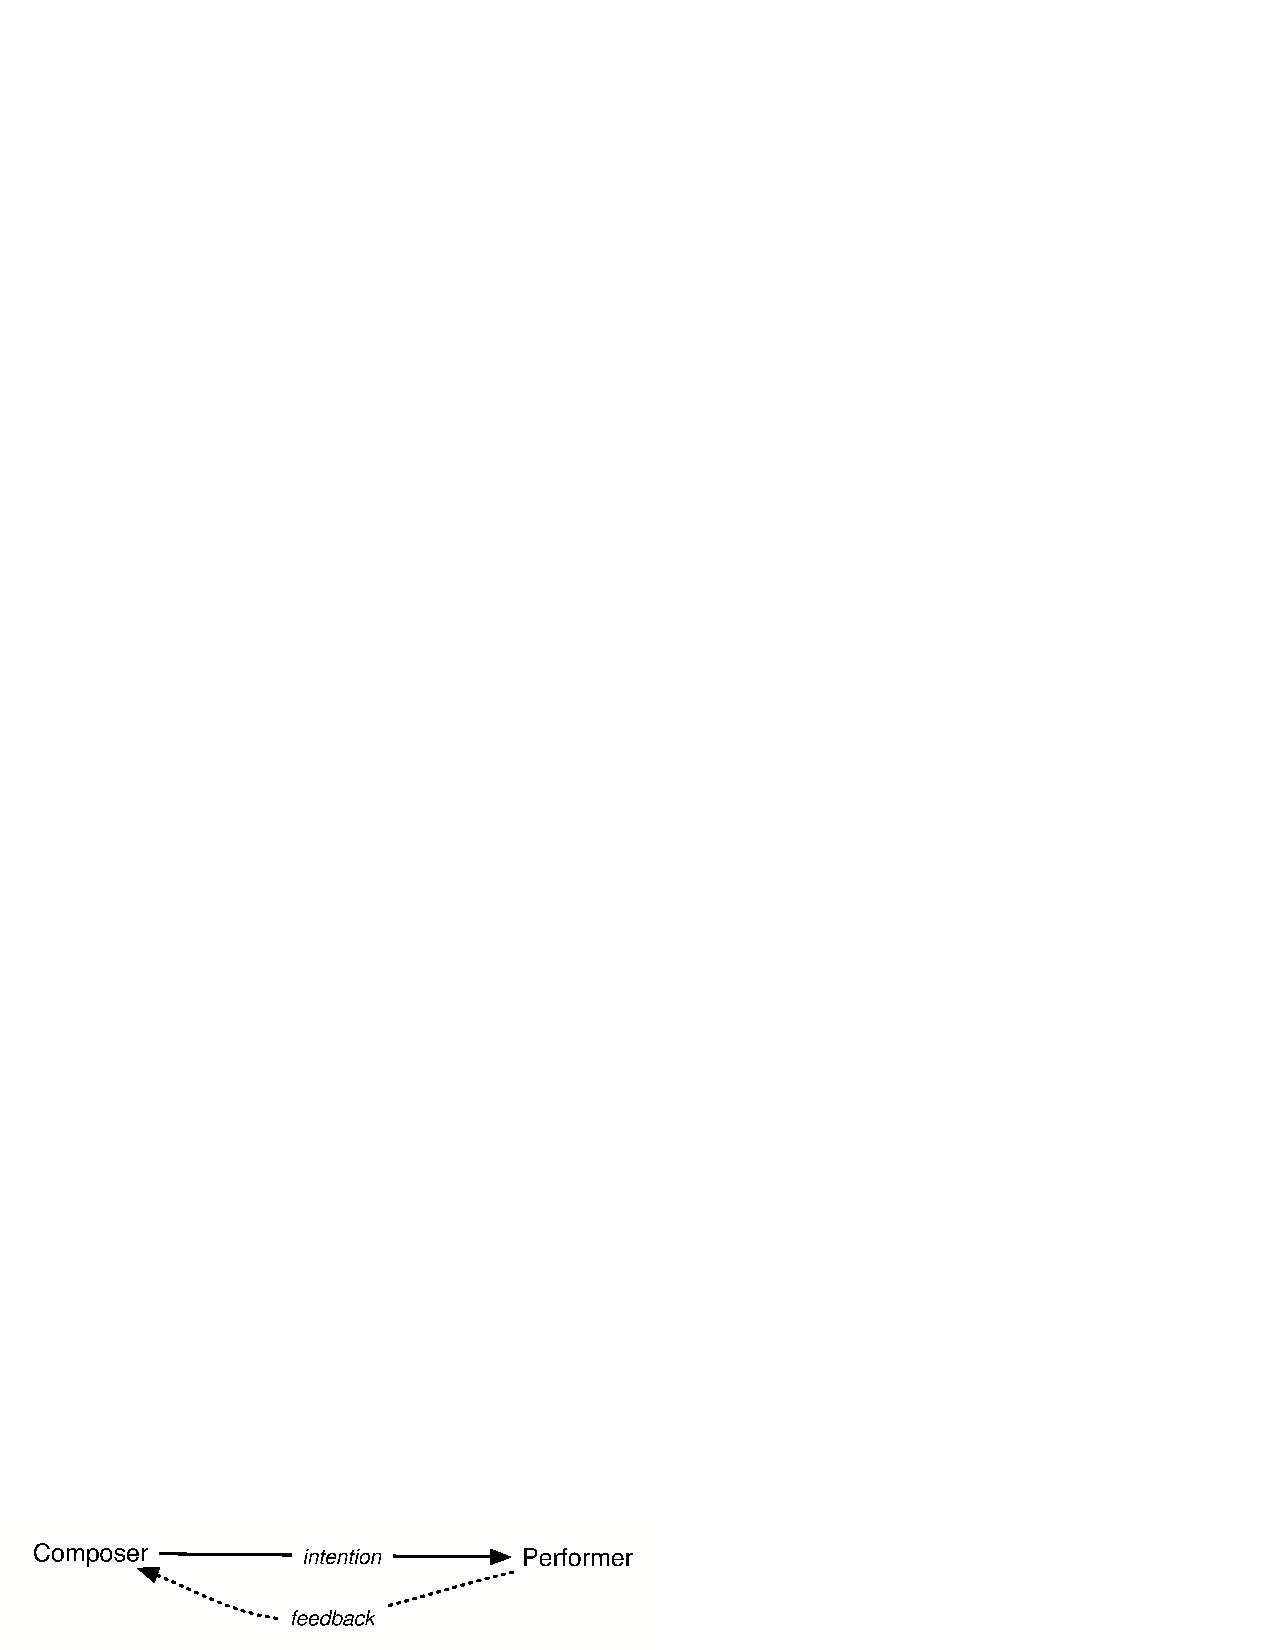
\includegraphics[width=1\columnwidth]{img/composer-performer}
  \caption{Intention in the documented session between S.{\"O}. and L.M..}
  \label{cmp_perf}
 \end{center}
 \end{figure}

 \begin{figure}[!t]
  \begin{center}
   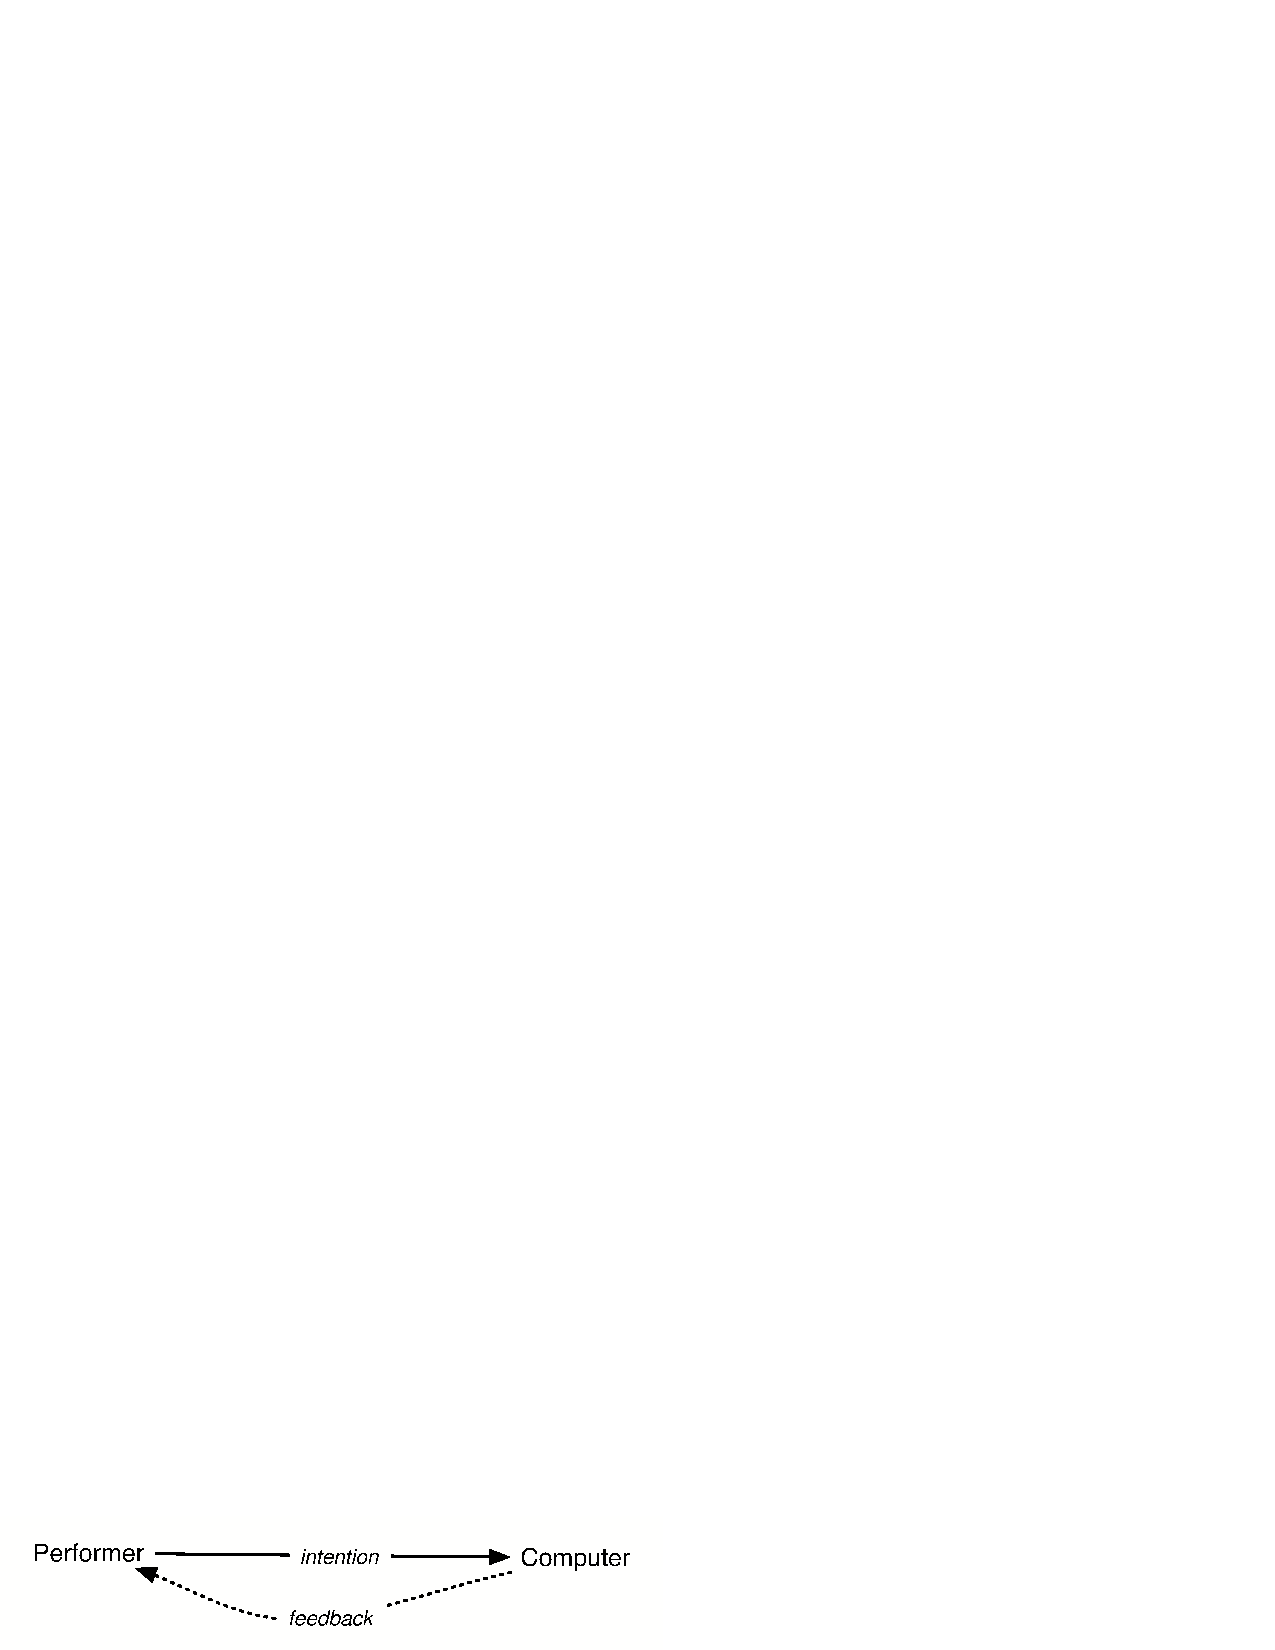
\includegraphics[width=1\columnwidth]{img/performer-computer}
   \caption{Intention in the performance in the suggested project. }
   \label{perf_cmp}
   \end{center}
 \end{figure}

The way the idea of the composer has been deconstructed in this study,
what remains of it is 'the one with the intention to create' (see Figure
\ref{cmp_perf}). 
On a higher level of intention, L.M. is the only agent
aiming at creating a musical work named ``\emph{Viken}''. S.{\"O}.'s higher level
intentions are towards performing L.M.'s work once it is finished and
contributing to the process of completing it.
%This is in accordance with Husserl's notion of
%'intentionality' or Derrida's idea of 'la diff\'{e}rance'. This is not
%to be confused with our term 'initiative' used in the graph. 
In the case of a performance of a mixed media work we find that the same
model transcribes to the level of performer and computer. The
flow of intention in the performance is on the performers side, the
computer being the responding part (see Figure
\ref{perf_cmp}). In other words, the attributes we
assign to the composer in the documented session belongs to the
interpreter at the stage of performance.

\subsection{Future work}
As already mentioned this study is intended to lay the ground for a
collaborative project - a piece for guitar and computer by Henrik Frisk
for Stefan {\"O}stersj{\"o}. It is our belief that thanks to the
research performed in this study we are both able to
enter this project with a slightly different view on our respective
practices. The concepts summarized in Sections 5.1-5.3 will form the
conceptual outline for the interaction between the performer and the
computer. This will give us a chance to further evaluate and refine or
denounce the principles sketched out in this study in the context of our
respective practices.


%This 'intention' is, in the model we are imagining for our project,
%transferred to the interpreter at the stage of performance.  

%%%
%%% The original style for the biblio.
%%%
% \bibliographystyle{chicago}

\bibliographystyle{apalike}
\small{
\bibliography{bibliography}
}

\end{document}